\documentclass[report]{vgtc}

\usepackage{mathptmx}
\usepackage{amsmath, bm}
\usepackage{graphicx}
\usepackage{caption}
\usepackage{float}
\usepackage{multicol}
\usepackage{times}
\usepackage{balance}
\usepackage{fancyhdr}
\usepackage[nooneline,hang,it,IT]{subfigure}
\usepackage{url}


%% Paper begins

\begin{document}
\large
	\begin{titlepage}
		\begin{center} 
			{\Huge GPU Accelerated Particle System} \\[1cm]

			{\LARGE Project in The Course TNCG14 Advanced Computer Graphics} \\[0.4cm]
			{\LARGE by August Ek and Oscar Johnson}
		\end{center}
	\end{titlepage}
	%% First page
	
\begin{abstract}
\\The aim of this project was to create a particle system mainly accelerated by the GPU. The system would then be used to render different effects. The system was accelerated using instance rendering and transform feedback leading to a huge performance gain. The particle system created was used to render different visualizations such as smoke, fire and rigid objects colliding with planes.   
\end{abstract}

\section{Introduction}
The graphics processing unit have a lot of potential which could be used in graphics calculations and even in arbitrary calculations surrounding these. One example well suited for this is a particle system. A particle system can be used in various applications. For example simulation of fluids, explosions and animation of hair. 
\\
The objective of this project is to extract the efficiency of the GPU. To demonstrate the power gained after GPU acceleration a particle system was implemented. Using particles to demonstrate gravitational physics and a simulation of smoke and fire with the use of perlin noise.
\\
This project uses opengl 4.1 which is a constraint. No compute shader is available to make non graphical calculations on the GPU. 

\section{Background and related work}
GPU:s primary goal have been to render graphical elements, however with time the GPUs functionality has been extended. Even non graphical calculations is possible on the GPU, and should often times be made there. Which could increase the performance by a great factor. The liability is now more with the programmer to make use of the GPU and moving much of the logic from the CPU to the GPU. This to fully exploit the efficiency of the computer.
\\
Even though compute shaders are not available in opengl 4.1 arbitrary calculations can be made on the GPU using a technique called transform feedback. This resolves the obstacle of not being able to do computations on the GPU. Another obstacle in GPU programming are the calls that has to be made from the CPU to GPU. These can create a bottleneck as well. Instancing is another technique which reduces the calls that has to be made. This basically creates a prototype of the particle instead of creating a new instance of each particle.
\\
There are some related articles that we have used as material. These articles include information about smoke simulation using perlin noise and are referenced in the report.
\section{Results}

\begin{figure}[H]
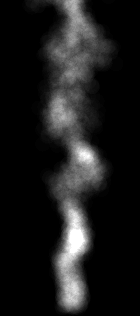
\includegraphics[height=200px]{img/smoke.png}
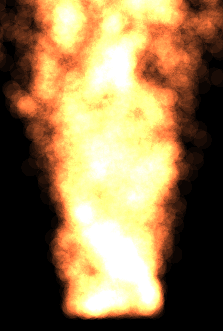
\includegraphics[height=200px]{img/fire.png}
\caption{Smoke and fire rendered with a noise based velocity field.}
\end{figure}


	\section{Implementation Details}	
	
	\subsection{Particles}

Each particle has two attributes: position and velocity. These two will need to be updated each frame before the particle is rendered to the screen. All of the particles are created at the start of the application and are then used to fill out the vertex buffer containing the positions and velocities a little by little.


\subsection{Calculating positions}
The new positions for the particles was calculated using transform feedback. This means that a shader was written that had the single purpose to calculate new positions for each particle. The resulting buffer from the shader was then used to draw the particles on the screen. Using this method gives a huge performance boost since all of the calculations could be moved from the CPU to the GPU, utilizing the parallel process power of the GPU and not relying on the few cores offered by the CPU.  The figure below shows how the main particle loop works.
\begin{figure}[H]
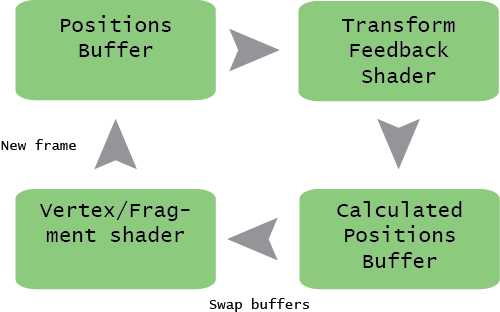
\includegraphics[scale=0.47]{img/transform.png}
\caption{Diagram describing the transform feedback. Positions and velocities are used as input to the transform feedback shader which produces new positions. These positions are then used to render the particles on the screen. }
\end{figure}

	\subsection{Rendering particles}
Instanced rendering was used to draw all of the particles with a single call to the GPU. This basically tells the GPU to render the same particle at different positions instead of render a different particle for each position. This offered a performance boost since the overhead related with making each API call would go from \(O(n)\) to \(O(1)\) per frame. 




	\subsection{Simulation}
Two different simulations were made to test the capabilities of the particle system. The first one uses classical mechanics to demonstrate particles colliding with planes and the second uses a noise based velocity field to simulate smoke and fire. 


	\subsubsection{Classical mechanics}

The physics implementation includes basic gravitational force. For each frame a new velocity and position is calculated due to gravity. 
A bounding box is surrounding the particles allowing implementation of collision detection. This is done with a simple posteori collision detection. Meaning if the particle moves outside the boundings, move it within the boundings in and calculate the new velocity. The new velocity is then calculated with the reflection formula for vectors.\\
If collision with the ground level would happen, the new velocity gets scaled with a number between 0.0 and 1.0. This is the coefficent of restitution, which represents the energy loss of the particle upon impact.\\
A calculation of the particles energy is done each frame. Using the particles mass, the gravity, distance to the bottom of the bounding box and velocity. This yields the kinetic and potential energy of the particle. If the energy value is less than a small given value, the particle is assumed still. To avoid unnecessary computation and vibrations at small energy values the velocity is set to zero and the position is assign previews value from then on.


	\subsubsection{Smoke}
To make a smoke simulation correct from a physical point of view, there is the need to solve the equations of Navier-Stokes. However, to get a visually realistic result, procedural methods could be used to create the vector field which moves the particles. This is easier to implement, more memory efficient and gives a result that looks realistic enough for this implementation.\\
The velocity field used was generated by using classic perlin noise\cite{stegu11}. The noise potential is simply a scalar field when implementing in 2D giving:
\begin{equation}
	\psi = \psi(x, y, z, time)
\end{equation}
x, y, and z are the positions of the particle, time is the elapsed time since the simulation started and \(\psi\) is the noise potential. Using the noise directly as the velocity field results in a field that diverges at certain areas thus producing a field with properties not desired for this type of simulation. Robert Bridson\cite{bridson07} proposes a solution to this by using the curl of the velocity field since one classic calculus identity is that \(\nabla \cdot (\nabla \times \mathbf{F}) = 0 \). Calculating the curl is done in the way:
\begin{equation}
	\mathbf{v} =  \nabla \times \psi
\end{equation}
Since only two dimensions were used, \(\psi\) were set to:
\begin{equation}
	\psi = (0, 0, \psi)
\end{equation}
giving:
\begin{equation}
	\mathbf{v} =(\frac{d\psi}{dy}, -\frac{d\psi}{dx})
\end{equation}
Which is the velocity of the particle at the given position and time.
The partial derivatives is then evaluated using simple finite differences with very small displacements. \\
The result is a divergence-free field which is essential to produce realistic velocity fields such  as those of smoke or water.  A comparison of the two noises can be seen below.
\begin{figure}[H]
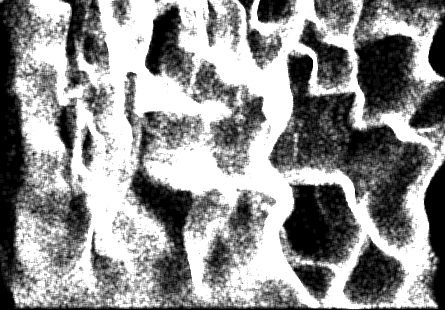
\includegraphics[scale=0.5]{img/noise.png}
\caption{Classic noise used as velocity field, notice the gutters where the particles tend to move.}
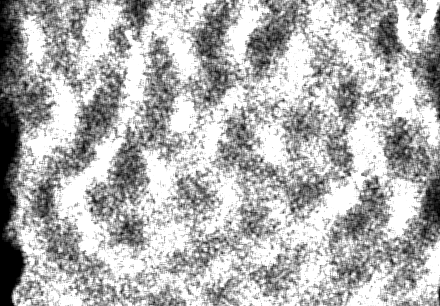
\includegraphics[scale=0.5]{img/curl-noise.png}
\caption{the curled noise used as vector field, this field is completely divergence - free.}
\end{figure}
\section{Conclusion}
The goal to implement a basic particle simulator was reached and by some extent exceeded. The simulator is using recent GPU techniques to boost the performance and using physics and vector calculus to simulate realistic scenarios. Transform feedback combined with instanced rendering removes the bottleneck of being limited to a low amount of particles. The system can easily handle hundreds of thousands of particles at smooth FPS rates even on low-end hardware. The particle system offers high modularity due to the fact that it’s very simple to replace the calculating vertex shader to give the particles a totally different pattern of motion thus simulating different phenomena.

\section{Future work and Improvements}
The smoke simulation could be improved in the way that the smoke respected boundaries giving the visual result that the smoke avoids some obstacles. This requires that the distance gradient of all obstacles is mixed with the noise-potential and we felt that we didn’t have the time for this feature. \\
Endless tweaking on parameters for the vector field could be done to create other visuals such as water. There is no real limit on how this could be done since the only goal is to create something aesthetically pleasant. Most of the work of this project had something to do with the motion of the particles and thus the calculations done in the vertex- and transform shader. A lot of work could be done in the fragment shader to drastically improve the visuals.\\
We can’t say that it wouldn’t be interesting to implement a physically accurate simulation with regards on the equations of Navier-Stokes. That simulation could then be used as reference to compare with the current one in aspects of performance and visual realism. \\
A graphical user interface could be implemented to easy swap between different simulations and the user could also be able to change some of the parameters such as: number of particles in the system, size of each particle and the location where the particles should be spawned. 


	

	%% Hardware used.
\def\arraystretch{1.5}%
	\begin{table}[h]
		\begin{tabular}{| ll |}
			\hline
			\textbf{Macbook Air 2013} & \textbf{Macbook Pro 2012} \\[0.75ex] %%\hline
			 1,3 GHz Intel Core i5  &   2,5 GHz Intel Core i5  \\[0.75ex]
			  8GB RAM & 8GB RAM    \\[0.75ex]
		 	 Intel HD Graphics 5000 &  Intel HD Graphics 4000   \\ [0.75ex]
			\hline
		\end{tabular}
	\end{table}	

	%%Benchmark
	

	\begin{table}[h]
		\begin{tabular}{l | r | r}
			  & 30 FPS & 60 FPS   \\[0.75ex] \hline
  			No Instancing, no Transform Feedback & 10 000 & 5000  \\[0.75ex]
  			Instancing & 300 000 & 100 000  \\[0.75ex]
			Instancing and Transform Feedback & 4 000 000 & 1 000 000 \\[0.75ex]


		\end{tabular}
	\end{table}	

\begin{thebibliography}{9}
\bibitem{stegu11}
  McEwan, I., Sheets, D., Gustavson, S. and Richardson, M. 2011,
  \emph{Efficient computational noise in GLSL}.\\
\url{http://webstaff.itn.liu.se/~stegu/jgt2012/article.pdf}

\bibitem{bridson07}
  Bridson, R., Hourihan, J. and Nordenstam, M. 2007,
  \emph{Curl-Noise for Procedural Fluid Flow}.\\
\url{http://www.cs.ubc.ca/~rbridson/docs/bridson-siggraph2007-curlnoise.pdf}
\end{thebibliography}




\end{document}
